\section{Automated Configuration of the AskoziaPBX Installation}
\label{sec:configuration}
This paragraph is about how the AskoziaPBX installations are automatically configured.
There is a complete configuration file in the appendix. First, the used configuration file
from Askozia is downloaded because the user should not have to reconfigure the whole box
including all accounts and the dialplan after every test. The target is to deliver
the Askozia box just like it was issued. So, there are three necessary steps which are described in the next chapters.
\begin{figure} [htbp]
\centering
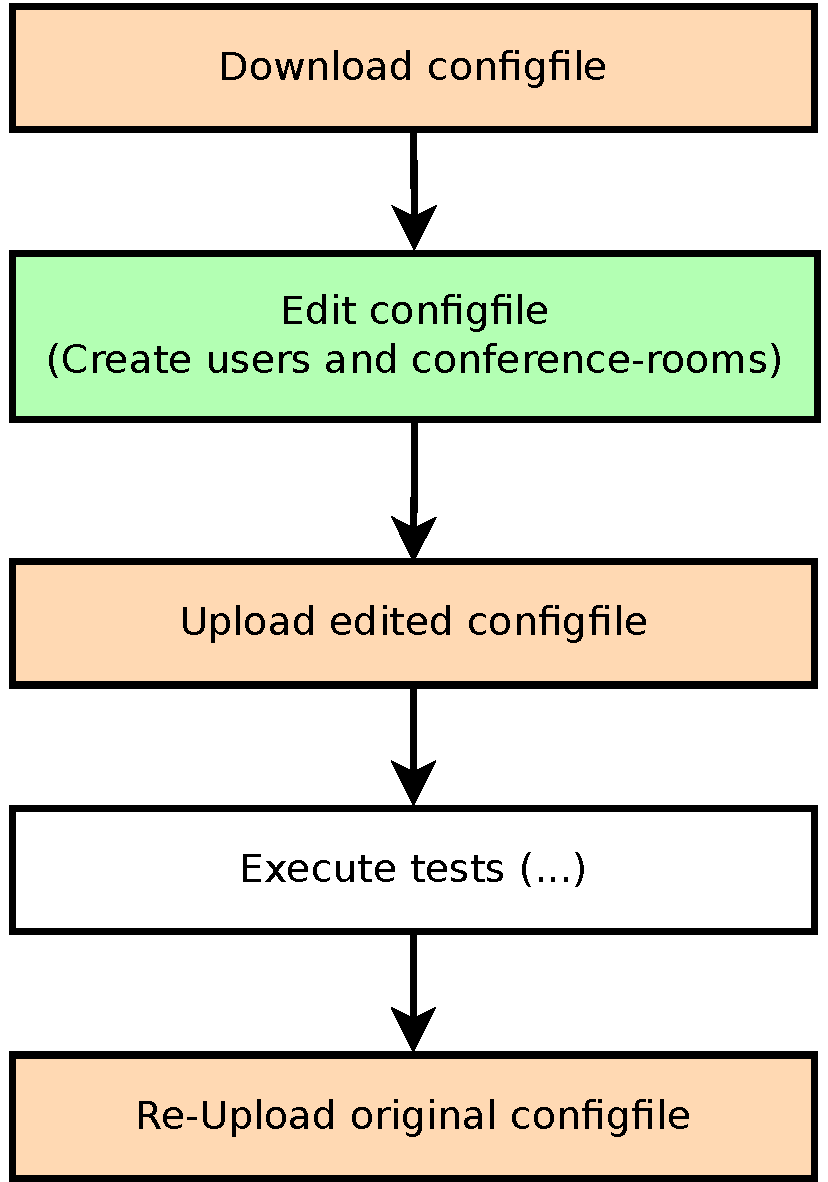
\includegraphics [width=7cm] {configuration-1}
\caption{Process of editing the Askozia-configuration file}
\end{figure}

%%%%%%%%%%%%%%%%%%%%%%%%%%%%%%%%%%%%%%%%%%%%%%%%%%%%%%
\subsection{Downloading/Uploading Configuration File}%
%%%%%%%%%%%%%%%%%%%%%%%%%%%%%%%%%%%%%%%%%%%%%%%%%%%%%%
For downloading the configuration file, it is necessary to send a HTML POST request to Askozia.
The useragent has to be authenticated as root and the content type must be ``multipart/form-data''.
For downloading the configuration file, the parameter ``Download'' has to be set.

\newpage In the performance test script, the following perl code is used to send this POST request:
\begin{lstlisting}[breaklines=true,label=code:config-post-request-download,caption={POST request for downloading the configuration file} ]
use HTTP::Request::Common;
use LWP;
my $ua = new LWP::UserAgent;
$ua->credentials ("$ask_ip:$ask_port",
	$ask_realm, "$ask_user" => "$ask_pw");
my $res = $ua->request (POST
	"http://$ask_ip:$ask_port/$ask_conf_page",
	"Content-Type" => "multipart/form-data",
	Content => [ Download => "1"]);
\end{lstlisting}

After executing this request, the following dataflow is to be expected:
\begin{figure} [h!]
\centering
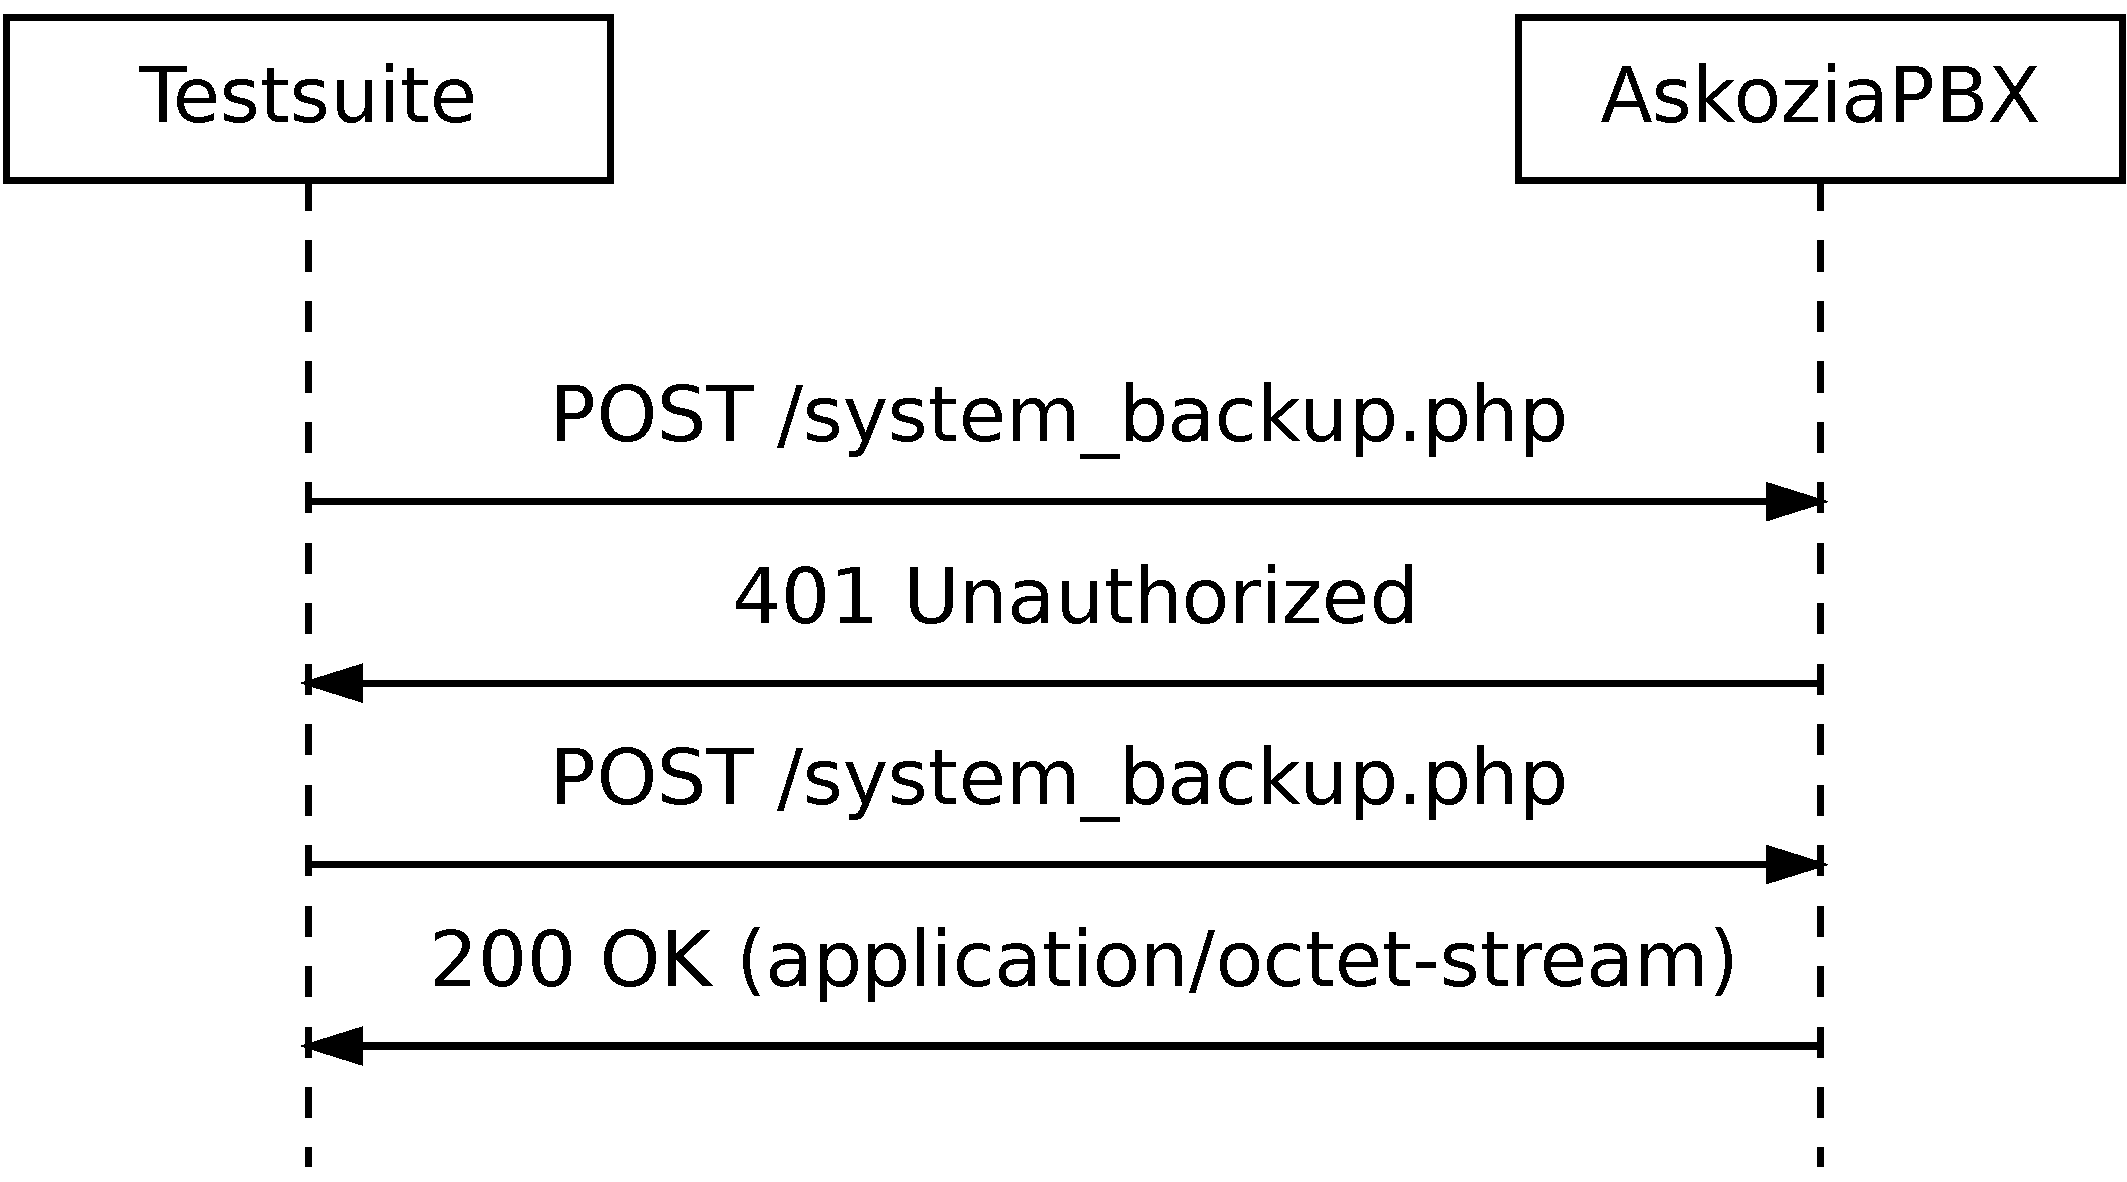
\includegraphics [width=11cm] {configuration-2}
\caption {Dataflow of configuration file download}
\end{figure}

The \texttt{200 OK} message sent by Askozia includes the configuration file in XML format. The XML file is saved with its original name
in the \texttt{./results/<testname>/} directory. Then, it is opened for reading to add the needed users and conference rooms
(see the next sections). When finished, the edited configuration file is saved with the original named followed by an \texttt{\_edited}
string. This edited configuration file is now uploaded to the AskoziaPBX as follows: \newpage

\begin{figure} [htbp]
\centering
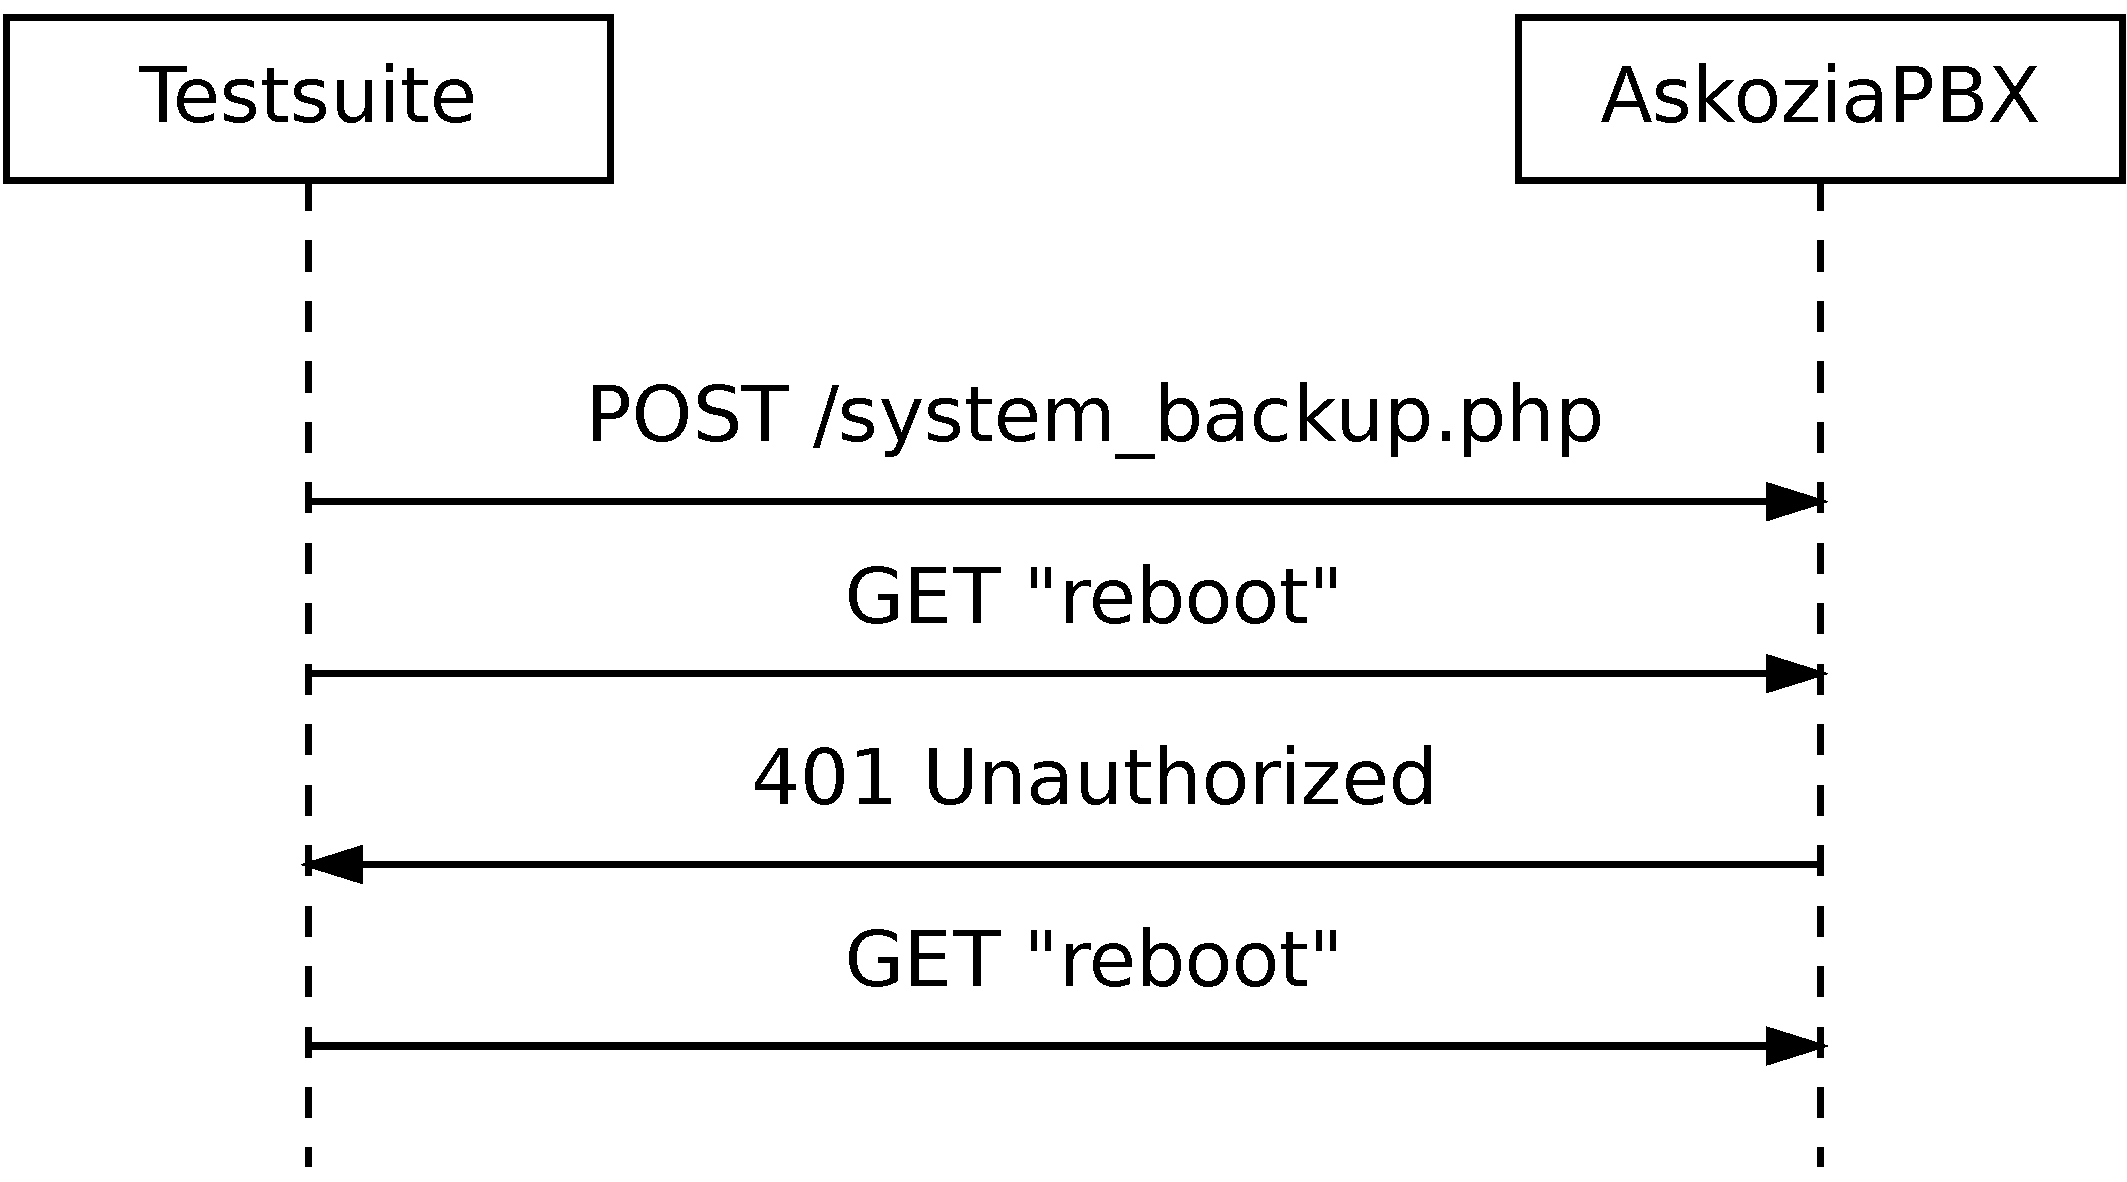
\includegraphics [width=11cm] {configuration-3}
\caption {Dataflow of configuration file upload}
\end{figure}

This dataflow is created by the following perl listing (\texttt{\$ua} and \texttt{\$res} are the existing variables declared and defined above):

\begin{lstlisting}[breaklines=true,label=code:config-post-request-upload,caption={POST request for uploading configuration file} ]
$res = $ua->request (POST
    "http://$ask_ip:$ask_port/$ask_conf_page",
	"Content-Type" => "multipart/form-data",
    Content => [ Restore => "1",
    conffile => [ $xml_configfile."_edited" ] ]);
\end{lstlisting}

After uploading the configuration file, the AskoziaPBX is rebooted.
This happenes automatically, but in this case, it is forced by an extra command sent as a GET request by using the webbased shell feature.
This manually forced reboot allows the script to ping Askozia and detect when it has finished rebooting.
Furthermore, it is now possible to wait some time (specified by using the \texttt{-{}-reboot-time} parameter)
to make sure that the PBX has enough time to start all services etc. after the reboot.
\begin{lstlisting}[breaklines=true,label=code:config-reboot,caption={Executing Askozia reboot} ]
my $ua = new LWP::UserAgent;
$ua->credentials ("$ask_ip:$ask_port",
    $ask_realm,	"$ask_user" => "$ask_pw");
$res = $ua->request (GET "http://$ask_ip:$ask_port/
    cgi-bin/ajax.cgi?exec_shell=reboot");
\end{lstlisting}


%%%%%%%%%%%%%%%%%%%
\subsection{Users}%
%%%%%%%%%%%%%%%%%%%
To execute the tests, it is necessary to add some test users to the AskoziaPBX installation.
The number of users depends on the parameters that were passed to the script when launching.
Here is a table of required users, the highest count will be added:

\begin{tabular}{|p{2cm}|p{12cm}|} \hline
	\textsc{Test type} & \textsc{Required users} \\ \hline \hline
	two-way & \texttt{= 2 * 2way-calls} (User A and B for each call) \\
	conf room & \texttt{= conf-calls-room * conf-rooms-room} \newline (``conf-calls'' users per ``conf-rooms'' conference rooms) \\
	conf call & \texttt{= conf-calls-call * conf-rooms-call} \newline (``conf-calls'' users per ``conf-rooms'' conference rooms) \\
	\hline
\end{tabular}

The script downloads the complete Askozia configuration file and searches for the end of the \texttt{sip} paragraph
Then, it adds its generated users. It is not checked whether the added phones already exist.
The template for adding users looks as follows, where \texttt{\_userno\_} is replaced by a three-digit integer that is incremented with each user:
\begin{lstlisting}[breaklines=true,label=code:config-user-template,caption={User template} ]
<phone>
<extension>_userno_</extension>
<callerid>Testuser _userno_</callerid>
<manualattributes>cXVhbGlmeT1ubw==</manualattributes>
<codec>alaw</codec>
<secret>_userno_</secret>
<uniqid>SIP-PHONE-_userno_</uniqid>
<language>en-us</language>
<ringlength>indefinitely</ringlength>
<natmode>yes</natmode>
<dtmfmode>auto</dtmfmode>
</phone>
\end{lstlisting}

%%%%%%%%%%%%%%%%%%%%%%%%%%%%%%
\subsection{Conference Rooms}%
%%%%%%%%%%%%%%%%%%%%%%%%%%%%%%
Just like the users, the needed conference rooms have to be added too.
The script searches for the end of the \texttt{conferencing} paragraph and adds its generated rooms.
The template looks as follows, where \texttt{\_roomno\_} is replaced by an integer that is incremented with each room:
\begin{lstlisting}[breaklines=true,label=code:config-room-template,caption={Conference room template} ]
<room>
<number>_roomno_</number>
<name>Default Conference</name>
<uniqid>CONFERENCE-ROOM-_roomno_</uniqid>
</room>
\end{lstlisting}

Conference rooms start with number 2000 (can be changed).
So, for a conference test that needs ten conference rooms, rooms from 2000 to 2009 are created.
